\chapter{Testing}
In order to be able to compare the results from this research, each demodulation technique considered needs to be tested and then the number of packets that the technique was able to successfully decode compared. From this analysis we will be able to see which techniques are effective and are able to decode relatively more packets as opposed to those that decode fewer. The testing for both the dedicated hardware and the software algorithms will be described in the corresponding sections below.

\section{Hardware Testing Setup}
The testing setup for the hardware is pretty simple since they are basically just black boxes that you need to supply the correct inputs to. Each piece of hardware has two connections, one is the radio port, and the other is the serial connection. As the name implies, the radio port is used to be able to interface with the radio. This port has connections for this such as transmit audio, receive audio, push-to-talk (ptt), vcc, and ground. A digram of the common radio port can be see in Figure \ref{RadioPortPinout} and found in any manual including those of Argent Data \cite{Systems2013}. Since this was common between multiple pieces of hardware, a simple break out board was created that allowed for a more universal audio transport mechanism of 3.5mm tip-ring-sleeve connectors, and also a 2.5mm barrel jack for power. This was much simpler than actually interfacing with a radio since the audio could just be played from a computer into the device; this device can be seen in Figure \ref{BreakOutBoard}. 

\begin{figure}
  \centering
	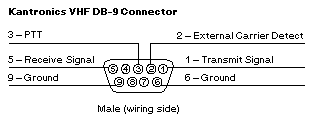
\includegraphics[width=0.75\linewidth]{images/RadioPortPinout.png} 
	\caption{Example Radio Port pin out for Kantronics, also consistent with others including Open Trackers \cite{Martin2014}.}
   \label{RadioPortPinout}
\end{figure}
\begin{figure}
  \centering
	\includegraphics[width=0.75\linewidth]{images/BreakOutBoard.png} 
	\caption{Break out board fabricated for hardware testing.}
   \label{BreakOutBoard}
\end{figure}

\section{New javaAX25 Demodulator Testing Framework}
Included within the javaAx25 suite was a testing application that could both generate and decode packets. However, it was limited to only being able to specify one audio file and one demodulation algorithm. Using this test file as a basis, a new testing application was created that allowed for the multiple algorithms to be compared side by side against multiple audio files with a single run of the application. In addition to the output being printed to the console, the output was also saved to a file. Having these features in the testing application allowed for a much more streamlined analysis of both all the algorithms and tuning individual algorithms. One very convenient aspect of programatically testing is that it is really easy to add a loop to try a range of tuning parameters and then look at the results to decide what is the best option. All the results listed in the following chapter are from the testing application / mechanism described here.
